%!TEX encoding = UTF-8 Unicode
% !TeX spellcheck = en_GB
%%%%%%%%%%%%%%%%%%%%%%%%%%%%%%%%%%%%%%
\chapter{The Standard Model Higgs boson }\label{chap:HiggsSM}
%%%%%%%%%%%%%%%%%%%%%%%%%%%%%%%%%%%%%%
\epigraph{	It's very nice to be right sometimes... it has certainly been a long wait.}{\textit{Peter Higgs }}

\section{Spontaneous symmetry breaking}
\par Before talking about symmetry breaking, we need to discuss the concept of symmetry in physics. Symmetry has an essential role in studying physical systems. It manifests not only as a geometric feature of physical objects but also in the dynamics of physical systems. For example, one can find symmetries in the equation of motion, Lagrangians/Hamiltonians and actions. The magnetisation of materials is a good example of the role that symmetry plays in describing physical behaviour. For instance, \textbf{paramagnetic} materials have a positive magnetic susceptibility~$\chi_B$ due to the random arrangement of their electrons' spins.  The paramagnetic material spins arrangement will therefore possess rotational symmetry. The material has no \textit{ preferred direction} in space~\cite{minlos2000introduction}. On the contrary, \textbf{ferromagnetic} materials with the electrons' spins aligned in a certain direction, will not have such symmetry as there will be a preferred direction, see~\autoref{fig:paravsferro}. 
%%%%
\begin{figure}[htpb!]
    \centering  
   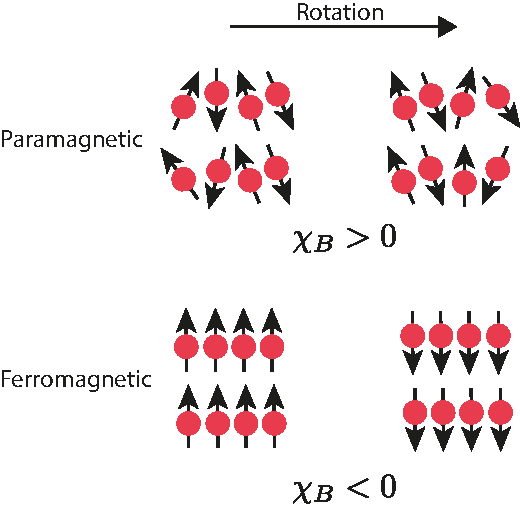
\includegraphics[width=0.36\linewidth]{./figures/ferrvspara}
    \caption{In paramagnetic materials, the spins are randomly distributed such that a rotation performed on the system will keep the spin distribution invariant. However, for ferromagnetic materials, where the spins are aligned in a single direction, the symmetry is broken, and the system has a preferred direction.}  \label{fig:paravsferro}
\end{figure}
%%%%
%%%%
\par In particle physics and quantum field theory, symmetry plays an essential role in the taxonomy and dynamics of elementary particles and their bound states, i.e. hadrons, cf.~\cite{osti_4008239,PhysRev.96.191}. There are two types of symmetries considered when studying elementary particles and their quantum fields: external and internal symmetries. The first is the symmetry of the spacetime background. Typically, this is a four-dimensional Poincar\'e symmetry. However, in some models, higher spacetime dimensions or non-flat geometries are considered. Though there is no current evidence of higher dimensions or indications of non-flat spacetime from colliders and cosmological observations~\cite{Zyla:2020zbs}. The second class of symmetries is internal symmetries stemming from the quantum nature of these particles/fields. Because their state is described by a \textbf{ray} in complex Hilbert/Fock spaces, internal symmetries are simply symmetries of rotations in these spaces that keep the action variation unchanged. Internal symmetries are usually described in terms of simple or product of simple \textbf{Lie groups}, e.g. $SU(N)$~\footnote{Gauge theories based on finite groups have been investigated in the literature, but their phenomenological significance is yet to be further investigated~\cite{Freed1993LecturesOT,dijkgraaf1990topological}}, and particles/fields will be arranged as multiplets in some representation of the groups. The rotations of the states could be parametrised by constants. In this case, the symmetry is called \textbf{global}, or fields of spacetime, where the symmetry is then called \textbf{local} or \textbf{gauged}.
%%%%
\par Gauge symmetries describe rotations in the state space that depend on spacetime, the generator of the gauge transformations could propagate between two spacetime points. This is the way particle/field interactions are described in quantum field theory. The generators of these gauge transformations are called gauge bosons, and they mediate the interactions between the particles/fields and transform under the adjoint representation of the gauge group. Hence, we observe that gauge symmetries are the basis of describing the fundamental interactions of nature, which we call \textbf{gauge theories}.
%%%%
\par An example of a gauge theory that is realised in nature is the \textbf{Standard Model}~(SM). Which is a gauge theory based on the group~$G_{\SM}:=SU(3)_C \otimes SU(2)_L \otimes U(1)_Y$. The first simple group is for the \textit{strong} interaction described by quantum chromodynamics~(QCD). The product of the two remaining groups~$SU(2)_L \otimes U(1)_Y$ forms the Weinberg-Salam \textit{electroweak}~(EW) model~\cite{salam1,salam2,PhysRevLett.19.1264}, where~$SU(2)_L$ describes the weak interaction which only couples to \emph{left handed} fermions and $U(1)_Y$ is the weak hypercharge~$Y$ gauge group, defined by the formula
\begin{equation}
    Y= 2(Q-T_3).
\end{equation}
Where $Q$ is the electric charge and $T_3$ is the third component of the weak isospin. A description of the matter content of the SM and their multiplicities with respect to~$G_{\SM}$ is shown in~\autoref{tab:thesm}
%%%%
\begin{table}[htpb!]
    \centering
    \begin{tabular}{ccc}
        \toprule
         Particle/Field& $G_\SM$ multiplicity& mass [\si{\GeV}] \\
         \midrule
         $Q = {u_L \choose d_L},{c_L \choose s_L},{t_L \choose b_L}$ & $(\irrep{3},\irrep{2},1/6)$ & $m_u=2.16\cdot10^{-3}$, $m_d=2.67\cdot10^{-3}$\\
         $U= u_R, s_R, t_R$ & $(\irrep{3},\irrep{1},2/3)$&$m_c=0.93\cdot10^{-2}$, $m_s=1.27$\\
         $D= d_R, s_R, b_R$ & $(\irrep{3},\irrep{1},-1/3)$&$m_t=172.4$, $m_b=4.18$\\
         \midrule
         $L = {\nu_{e,L} \choose e_L},{\nu_{\mu,L} \choose \mu_L},{\nu_{\tau,L} \choose \tau_L}$ & $(\irrep{1},\irrep{2},-1/2)$ & $m_e=0.511\cdot10^{-3}$, $m_\mu=1.05\cdot10^{-2}$\\
         $E= e_R, \mu_R, \tau_R$ & $(\irrep{1},\irrep{1},-1)$&$m_\tau=1.77$,$m_\nu=$??\\
         \midrule
         $g/G^A_\mu,\,\,\, A=1\dots 8$ &$(\irrep{8},\irrep{1},0)$&$ 0.0$\\
         $\gamma/A_\mu$ &$(\irrep{1},\irrep{1},0)$&$ 0.0$\\
         $W^\pm_\mu$ &$(\irrep{1},\irrep{3},0)$&$ 80.379$\\
         $Z_\mu$ &$(\irrep{1},\irrep{3},0)$&$ 91.1876$\\
         \midrule
         $h$ &$(\irrep{1},\irrep{2},1/2)$&$ 125.10$\\
        \bottomrule
    \end{tabular}   
        \caption{The SM constituents, their multiplicities with respect to the SM gauge group ~$G_{\SM}:=SU(3)_C \otimes SU(2)_L \otimes U(1)_Y$ and masses. The mass of the neutrinos $\nu$ is zero according to the SM prediction, but observations suggest that they are massive, and only the difference between the three masses is known~\cite{Capozzi:2016rtj}. The values of the masses are taken from the Particle Data Group~(PDG)~\cite{Zyla:2020zbs}, and used throughout this thesis.}\label{tab:thesm}
\end{table}

%%%%
%%%%
\par The SM has been very successful at describing particle interactions even when challenged by numerous precision tests at LEP and SLD~\cite{ALEPH:2005ab,SLD:2000jop,Group:2012gb,ALEPH:2013dgf} and later at D\O~\cite{2011baz} and the LHC~\cite{CMS:2014mgj,ATLAS:2017rzl} Nevertheless, it fails to describe the ground state if only the fermion and gauge sectors are considered. The reason for this shortcoming is that the $W^\pm$ and $Z$ bosons have a mass, this violates the EW gauge symmetry. This can be easily seen by looking at the mass term of a spin 1 field $B^A_\mu$
\begin{equation}
    \mathcal{L} = m_B B^{A,\mu}B^A_\mu,
\end{equation}
and performing an $SU(N)$ gauge transformation 
\begin{equation}
    B^A_\mu \to B^A_\mu+\partial_\mu \Lambda ^A+g \,\varepsilon^A_{BC} B^B_\mu \Lambda^C.
\end{equation}
We see that the mass term is invariant under these transformations.
Secondly, because the SM is a chiral theory, as only left-handed fermions would be doublets under~$SU(2)_L$, the Dirac mass term
\begin{equation}
    \mathcal{L}_{\mathrm{D}} = m_D \bar \psi_L \psi_R+ \hc,
\end{equation}          
cannot be a singlet under~$SU(2)_L$, hence also violating the EW symmetry. Despite quark and lepton masses being forbidden by the EW symmetry, we indeed observe that they do have a mass, and since they also carry charges this mass has to be a Dirac mass. 
\par In order for the EW model to be consistent at the ground state like it is in the interaction states. A mechanism for spontaneous symmetry breaking going from an interaction state to the vacuum ought to be introduced. 
%%%%%%
\subsection{Nambu-Goldstone theorem}
%%%%%%%
Coming back to the example of the paramagnetic-ferromagnetic materials, when heated above a certain temperature, known as the~\textbf{Curie Temperature}~$T_C$ will undergo a phase transition and become paramagnetic~(losing their permanent magnet property), in the mean-field theory approximation the magnetic susceptibility is related to the temperature of the metal via the relation
\begin{equation}
    \chi_B \sim (T-T_C)^{-\gamma},
\end{equation}  
where $\gamma$ is a critical exponent. We see that if the metal temperature $T>T_C$ the metal is in an~\textit{disordered phase} and when $T<T_C$ it is in the~\textit{ordered phase},i.e. $\chi_B$ is the \textbf{order parameter} of this system. At the Curie temperature, the system will be at the~\textit{critical point} where the susceptibility is divergent. The exponent $\gamma$ is not used to describe the system at the critical point. There is a ``pictorial'' description of the metal at the critical point which is helpful in picturing the Goldstone theorem. Starting at $T>T_C$, the metal would be in a paramagnetic phase, where the spins are randomly arranged. As the temperature becomes lower and lower, thermal fluctuations start to lessen.  One or more regions of the metal, some of the spins will start to get aligned With continued cooling, nearing $T_C$, these turned spins will affect their neighbours turning them into their directions. At the critical point $T=T_C$, the system behaves in a peculiar manner, when one would see regions of spins in ``up'' and others in ``down'' directions. The system will resemble a fractal of these regions, becoming scale-invariant. Additionally, waves of oscillating local magnetisation will propagate. These waves, or spinless quasiparticles (called \textbf{Magnons}) are Goldstone bosons emerging from spontaneous symmetry breaking. Which will manifest at $T<T_C$ as the spins will be  arranged in a certain single direction and the metal becomes ferromagnetic.
\begin{theorem}[Nambu-Goldstone]
    When a continuous symmetry has a conserved currents but broken in the ground state~(vacuum) is called to be spontaneously broken. There is a scalar boson associated with each broken generator of this spontaneously broken symmetry. The modes of these bosons are fluctuations of the order parameter.
\end{theorem}
This theorem first emerged from condensed matter physics, particularly superconductors~\cite{PhysRev.117.648,goldstone}. However, it soon got applied to relativistic quantum field theories~\cite{PhysRev.127.965}.
%%%%%%
\section{The Higgs mechanism}
%%%%%%
In order to solve the aforementioned shortcomings of the Weinberg-Salam model, Nambu-Goldstone theorem has been first proposed by P.~W.~Anderson~\cite{PhysRev.130.439}. However, the way that Anderson formulated his theory was unfamiliar to particle physicists and used a non-relativistic picture to illustrate how photons could gain mass in an electron plasma with a plasma frequency $\omega_{p}$ 
\begin{equation}
    m_\gamma^{\mathrm{plasma}} =\frac{\hbar \omega_p}{c^2}
\end{equation}
Later on, a theory that explains the mass generation of the EW gauge bosons has been published in an almost simultaneous manner by R.~Braut~ and F.~Englert~\cite{PhysRevLett.13.321}, P.~Higgs~\cite{PhysRevLett.13.508} and G.~Guralnik, C.~R.~Hagen, and T.~Kibble~\cite{PhysRevLett.13.585,Guralnik:2009jd}\footnote{All of these authors have contributed to the theory of SM spontaneous symmetry breaking~(SSB). By calling it the ``Higgs'' mechanism or boson. I, by no means, have intended to ignore the role played by the rest, rather, I wanted to stick the most widely-used terminology in the field.}.
The Higgs mechanism starts by considering the spontaneous symmetry breaking~(SSB) of the EW sector of the SM via the pattern
\begin{equation}
    SU(2)_L \otimes U(1)_Y \longrightarrow U(1)_{Q} 
\end{equation}
This is  achieved by the vacuum expectation value~(vev) of a complex scalar field $\phi\sim (\irrep{1},\irrep{2},+1/2)$, with the Lagrangian 
\begin{equation}
    \mathcal{L} = D_\mu \phi^* D^\mu \phi -V,\;\;\;\;\;\; V:= \mu^2  \phi^* \phi +\lambda (\phi^* \phi)^2,
    \label{higgspot}
\end{equation}
 were $\phi$ is given explicitly by 
 \begin{equation}
  \phi = \begin{pmatrix}
      \phi^1 + i \phi^2\\  \frac{1}{\sqrt{2}}(h+v)-i \phi^3
  \end{pmatrix}
\end{equation}
The covariant derivative 
\begin{equation}
    D_\mu= \partial_\mu -ig_2\frac{\sigma_a}{2}W^a_\mu-ig_1\frac{1}{2} B_\mu,   
\end{equation}
dictates the coupling between the Higgs field and the EW gauge bosons and~$g_3$, $g_2$ and $g_1$ are, respectively, the coupling constants of 
${ SU(3)_C}$,  ${ SU(2)_L}$ and  ${ U(1)_Y}$.  
 The minimum of the scalar potential is then obtained by
 \begin{equation}
\frac{\partial V}{\partial \phi} \mid_{\phi\to v} = 0,
\end{equation}
which for a tachyonic mass~$\mu^2 < 0$ will have a real non-vanishing values~$v$ corresponding to the vev of this field~$\langle \phi \rangle ={0\choose \frac{v}{\sqrt{2}}}$.\\
According to Nambu-Goldstone theorem, the three broken generators of~$SU(2)_L \otimes U(1)_Y$ will become massive, and they are the $W^\pm$ and $Z$ bosons, while the photon will remain massless. We will have three massless Goldstone bosons $ G^\pm=\frac{1}{2} (\phi^1\pm i\phi^2) $ and $G^0=\phi^3$ that are ``eaten'' by the aforementioned massive photons. Where they become the longitudinal polarisations of $W^\pm$ and $Z$ boson. In order to see this more concretely, we start by looking at the terms of the EW Lagrangian where the field $\phi$ couples to the gauge bosons, in the unbroken phase
\begin{equation}
   D_\mu \phi^* D^\mu \phi = \frac{1}{2} |\partial_\mu \phi|^2 + \frac{1}{8}g_2^2|\phi|^2|W_\mu^1+iW_\mu^2|^2
   + \frac{1}{8}|\phi|^2 |g_2 W_\mu^3- g_1 B_\mu|^2
   \label{ewhiggs_ub}
\end{equation}
After SSB, we write the gauge bosons in the mass basis~
\begin{align}
W_\mu^\pm &= \frac{1}{\sqrt{2}} (W^1_\mu\pm iW^2_\mu), \nonumber \\
Z_\mu &= \frac{1}{\sqrt{g_1^2+g_2^2}} \left(g_2 W^3_\mu-g_1B_\mu\right), \\
A_\mu &= \frac{1}{\sqrt{g_1^2+g_2^2}} \left(g_2 W^3_\mu+g_1B_\mu\right). \nonumber
 \end{align}
 From this, the electric change is identified as the coupling constant to the photon~$A_\mu$ 
 \begin{equation}
     e=\frac{g_1}{\sqrt{g_1^2+g_2^2}}.
 \end{equation}
 It is useful to define~\textbf{Weinberg angle}~$\theta_W$, an important EW parameter relating the electric charge to the weak coupling~$g_2$ 
 \begin{equation}
     \sin \theta_W = \frac{e}{g_2} \approx 0.231214,
 \end{equation}
 typically the $\sin$ and $\cos$ of the Weinberg angle are denoted by $s_W$ and $c_W$, respectively. \\ We use the unitary gauge, to absorb the Goldstone bosons into the $W^\pm$ and $Z$ longitudinal polarisations. In this gauge the Higgs doublet can be written as
\begin{equation}
    \phi \to \begin{pmatrix}
       0\\  \frac{1}{\sqrt{2}}(h+v).
    \end{pmatrix}, \,\,\,\,\,\,\,\, v= 246\, \mathrm{GeV}.
    \label{unitaryhiggs}
  \end{equation}
With these substitutions, one can read off the masses of the gauge bosons their bilinear terms in~\eqref{ewhiggs_ub}
\begin{align}
    m_W =& \frac{vg_2}{2} & m_Z&=\frac{v}{2}\sqrt{g_1^2+g_2^2} & m_A &= 0.
\end{align}
Since $\phi$ is a complex doublet. We have seen that it has four components,  and three of them correspond to the Goldstone bosons, thus one remains physical~$h$ which is what we now identify with the ``Higgs boson'' discovered in the Summer of 2012~\cite{CMS:2012qbp,ATLAS:2012yve}. The couplings between  the Higgs and the electroweak bosons is related to their mass via the vev 
\begin{align}
    g_{hVV} =& \frac{2 m_V^2}{v}, & g_{hhVV}=& \frac{2 m_V^2}{v^2}.
\end{align}
By substituting~\eqref{unitaryhiggs}, into the Higgs potential~\eqref{higgspot} one can write the mass of the physical Higgs boson in terms of the vev
\begin{align}
  m_h =\sqrt{2 \lambda} v .
\end{align}
The physical Higgs mass is related to the $\mu$ parameter via the relation
\begin{align}
	m_h ^2 =-2 \mu^2,
\end{align}
One can see that the mass term after SSB changes its sign, characterising the order-parameter for this system,  analogous to the magnetic susceptibility for the magnetisation of materials example. 
One could also identify the self-couplings of~$h$, the trilinear and quartic couplings 
\begin{align}
    g_{hhh}&=3\lambda v =3\frac{m_h^2}{v}, & g_{hhhh}&= 3 \lambda = 3\frac{m_h^2}{v^2}.
\end{align}
%%%
\section{Yukawa interaction}
It is possible to also use the Higgs vev to give fermions their masses by introducing a Yukawa-interaction terms, first introduced by S. Weinberg~\cite{PhysRevLett.19.1264}
\begin{equation}
    \mathcal{L}_{\mathrm{Yuk}}= -y_{e} \, \bar{L} \, \phi \, E 
- y_{d} \, \bar{Q} \, \phi \, D
- y_u \, \bar{Q} \, \tilde{\phi} \, U   \ + \hc,
\label{lag-yuk}
\end{equation}
with $ \tilde{\phi}= i\sigma_2 \phi$ and $ y_e, y_d, y_u$ are $3\times 3$ matrices. These matrices are free parameters in the SM. As the Higgs boson acquires a the vev, the fermions will acquire a mass $m_f= vy^\prime_f$ and the Higgs boson coupling to the fermions is given by
\begin{equation}
	g_{h\bar{f}f} = \frac{m_f}{v},
\end{equation}
 and the Yukawa matrices will be fixed in the mass basis ~$y^\prime_f$ by measurements of the fermion masses.\\  Leptonic Yukawa matrix is diagonal, with a degeneracy between the flavour and masses basis, this manifests as lepton family number conservation~(the lepton family operator commutes with the Hamiltonian.). However, for the quarks, the situation is more complicated. One can rotate these matrices to the mass basis via a bi-unitary transformation via the unitary matrices~$ \mathcal{V}_Q, \mathcal{U}_Q$ for $ q= u,d$
\begin{equation}
    y_{q} \longrightarrow y^\prime_f= \mathcal{V}^\dagger_{q} \,y_q\, \mathcal{U}_{q} = \text{diag}\left(m_{q_1}, m_{q_2},m_{q_3}\right).
\end{equation}
However, the is no degeneracy here as the Hamiltonian does not commute with the quark flavour operator. This is because the transformation matrices for the up and down-type quarks are not the same.  The charged EW quark currents contains flavour mixing described by the Kabibbo-Kobayashi-Maskawa~(CKM) matrix~\cite{PhysRevLett.10.531,10.1143/PTP.49.652}. More details on the flavour sector of the SM is discussed in~\la{Update the section}\\
\autoref{fig:SMcouplings} shows all the SM couplings' strengths, with the thickness of the chord is proportional to the strength of the coupling, on can see the Higgs couplings in orange. 
%%%%
\begin{figure}[htpb!]
    \centering
    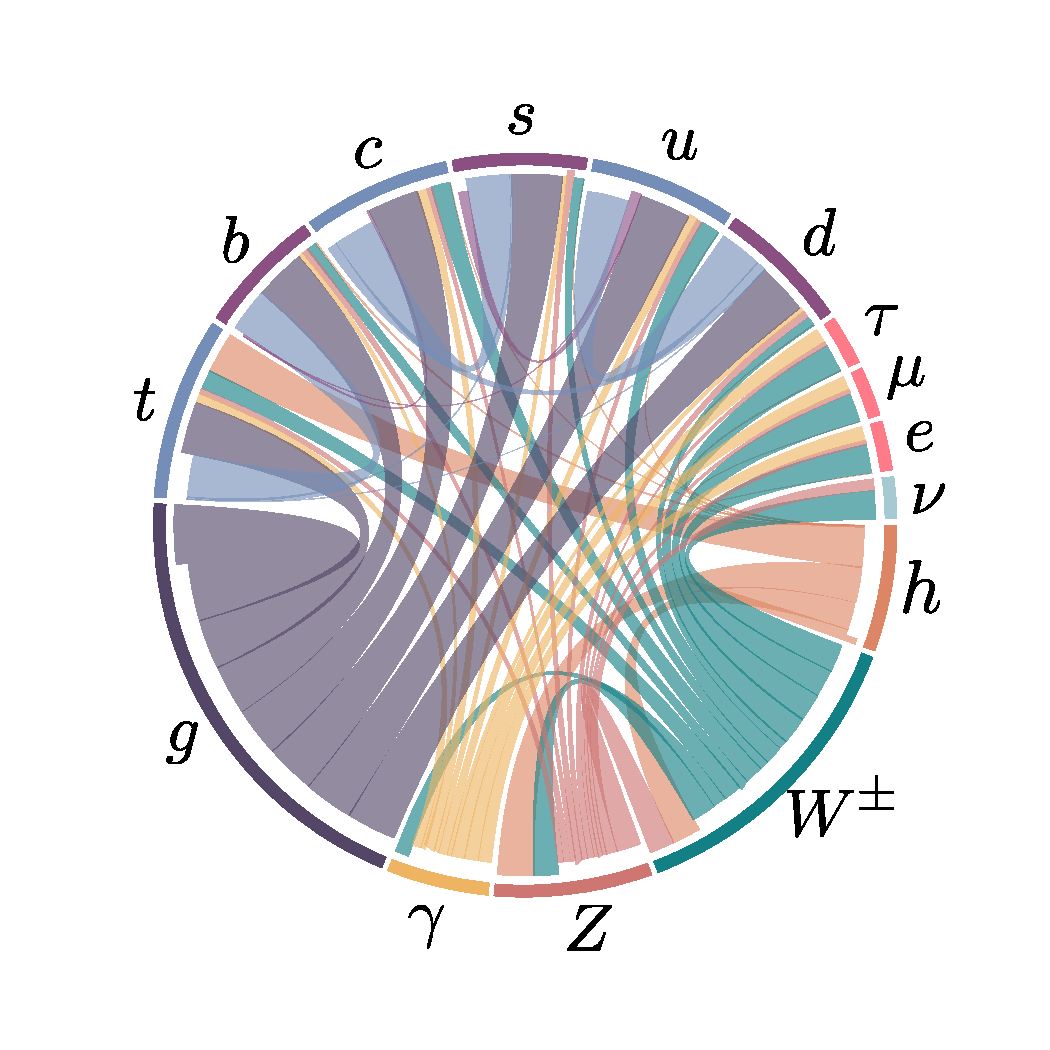
\includegraphics[width=\linewidth]{./figures/SM}
    \caption{A chord diagram showing the SM couplings, with the coupling strength illustrated by the chord thickness. Higgs couplings are coloured in orange.}  \label{fig:SMcouplings}
\end{figure}
%%%%
%%%%
\section{The Higgs and EW precision observables}
\par Higgs physics is intertwined with the EW sector for example, the Higgs vev is determined from Fermi's constant~$v =(\sqrt{2}G_F)^{-1/2}$, and is fixed by muon lifetime measurements, and comparing it with the theoretical predictions~\cite{PhysRev.101.866,PhysRev.113.1652,Mohammad:1976qd,PhysRevLett.82.488} 
\begin{equation}
    \tau_\mu^{-1} = \frac{G_F^2 m_\mu^5}{192\pi^3}\left(1-\frac{8 m_e^2}{m_\mu}\right) \left[1-1.810\frac{\alpha}{\pi}+(6.701\pm0.002)\left(\frac{\alpha}{\pi}\right)^2\right],
\end{equation}
which leads to the numerical value of $G_F$~\cite{Zyla:2020zbs}
\begin{equation}
    G_F=1.1663787(6) \cdot 10^{-5} \si{\per\GeV\squared},
\end{equation}
given the value of the fine structure constant~$\alpha^{-1} =137.03599976 (50)$. 
\par Another important EW precision observable~(EWPO) is the ratio between the $W$ and $Z$ masses
\begin{equation}
    \rho = \frac{m_W^2}{c_W^2m_Z^2}.
\end{equation}
At leading order, this parameter is equal to unity in the SM. The $\rho$ parameter depends on the representation of the scalar sector of the EW model having $\phi_i$ scalars with $T_i$ weak isospin and $T_{3,i}$ being its third component, and a vev $v_i$, via the relation~\cite{ROSS1975135,Djouadi:2005gi}
\begin{equation}
    \rho =\frac{\sum_i [T_{i}(T_{i}+1)-T_{3,i}^2]v_i^2}{2\sum_i T_{3,i}^2v_i^2}.
    \label{rhohiggs}
\end{equation}
From~\eqref{rhohiggs} one can see that a real triplet scalar, for instance, would not fit the experimental EW measurement of $\rho$. Hence, a complex doublet is the simplest scalar possible for the EW symmetry breaking, and the Higgs boson was expected to be seen almost four decades before its discovery. However, radiative corrections to the EW gauge bosons mass from vacuum polarisation diagrams could potentially cause $\rho$ to deviate significantly from unity.  This is not the case, as the experimentally measured value of~$\rho$~\cite{Zyla:2020zbs}
\begin{equation}
    \rho_{\text{exp}} = 1.00038 \pm 0.00020
    \label{eq:rhoexp}
\end{equation}
Additionally, it is possible to think of an extended Higgs sector, where there are multiple scalars with different $SU(2)_L$ multiplicities. Or, a composite Higgs sector, where the Higgs boson is a pseudo Nambu-Goldstone boson, cf.~\cite{Dugan1985AnatomyOA,Hill:2002ap}. How can such models be built assuring the $\rho$ parameter is protected from change ? The answer to this question lies in a symmetry of the Higgs Lagrangian known as custodial symmetry. 
\subsection{Custodial symmetry}
After SSB, a residual global symmetry known as the custodial symmetry protects the $\rho$ parameter from obtaining large radiative corrections at higher orders in perturbation theory.  This symmetry must be kept in extended or composite Higgs models. This symmetry can be seen by rewriting the Higgs potential as
\begin{equation}
	V = \frac{\lambda}{4} \left(å \phi_1^2+\phi^2_2+\phi_3^2+\phi^2_4 -2 \mu^2\right)^2.
\end{equation}
This potential is invariant under $SO(4)\simeq SU(2)_L \otimes SU(2)_R$ rotations. However, when the Higgs field squires a non-vanishing vev,  $ \phi_4 \to h+v$, the potential becomes
 \begin{equation}
 	V = \frac{\lambda}{4} \left( \phi_1^2+\phi^2_2+\phi_3^2+ h^2+2vh+v^2 -2 \mu^2\right)^2,
 \end{equation}
which is only invariant under  $SO(3)\simeq SU(2)_V$ transformations, the diagonal part of the original group. This global SSB pattern comes alongside the EW SSB of the gauge group $SU(2)_L \otimes U(1)_Y$ as global $SU(2)_L$ is itself the gauged $SU(2)_L$  group. Additionally the $T^3$ component of the ~$SU(2)_R$ global group is the gauged $U(1)_Y$ and the~$T^3$ component of the custodial group~$SU(2)_V$ is gauged as well and identified to be the electric charge operator, i.e. the generator of $U(1)_Q$. 
\begin{equation}
	\underbrace{SU(2)_R}_{{\color{myblue} \supset\, U(1)_Y}} \otimes \overbrace{SU(2)_L}^{{\color{myblue} \text{gauged}}} \longrightarrow \underbrace{SU(2)_V}_{{\color{myblue} \supset\, U(1)_Q}} .
\end{equation}
This pattern indicates that the symmetry is already broken by the gauging of the diagonal part of $SU(2)_R$ ~(the hypercharge). The custodial symmetry is only \emph{approximate} in the limit of $ g_1 \to 0$, and $\rho=1$ is a consequence of $g_1\neq 0$ . The symmetry breaking pattern $\irrep{2} \otimes \irrep{2} = \irrep{3} \oplus \irrep{1}$ also allows us to identify the Goldstone bosons as the custodial triplet and the physical Higgs~$h$ as the custodial singlet, explaining the electric charge pattern they have.   \\
 We could use the isomorphism between the special orthogonal and special unitary groups to parametrise the Higgs doublet as an 
$SU(2)_L \otimes SU(2)_R$ bidoublet 
\begin{equation}
	\mathcal{H} =(\tilde{\phi} \,\,\, \phi) = \frac{1}{\sqrt{2}}\begin{pmatrix}
		\phi_4-i\phi_3 & \phi_1+i\phi_2 \\
		 \phi_1-i\phi_2 & \phi_4+i\phi_3
	\end{pmatrix},
\end{equation}
with the bi-unitary transformations
\begin{equation}
	\mathcal{H} \longrightarrow \mathcal{U}_L \mathcal{H} \mathcal{U}^\dagger_R
\end{equation}
which leaves any traces of the form $\mathrm{Tr}(\mathcal{H}^\dagger\mathcal{H})$, invariant. The Higgs potential could be rewritten in terms of the bidoublet 
\begin{equation}
	V = -\frac{\mu^2}{2} \mathrm{Tr}(\mathcal{H}^\dagger\mathcal{H} + \frac{\lambda}{4}\left(  \mathrm{Tr}(\mathcal{H}^\dagger\mathcal{H} \right) ^2
\end{equation}
The vev is hence written in this representation as 
\begin{equation}
\langle \mathcal{H} \rangle  = \frac{v}{\sqrt{2}}\, \mathbb{1}_{2\times 2}.
\end{equation}
We can also look at the Yukawa sector, and observe that in the case where $ y_u =y_d =y $, we can also write the left-handed and right-handed quarks  as $SU(2)_L \otimes SU(2)_R$  bidoublets and $SU(2)_R$ doublets, respectively. Hence, the quark part of the Yukawa Lagrangian in~\eqref{lag-yuk} becomes
\begin{equation}
	\mathcal{L}_{yuk} \supset \frac{y}{\sqrt{2}}  (\bar u_L\,\,\, \bar d_L)  \begin{pmatrix}
		\phi_4-i\phi_3 & \phi_1+i\phi_2 \\
		\phi_1-i\phi_2 & \phi_4+i\phi_3  
	\end{pmatrix}  \begin{pmatrix}  u_R \\ d_R	\end{pmatrix} ,
\end{equation}
which is invariant under custodial transformations, but when~$ y_u \neq y_d$, this Lagrangian term breaks custodial symmetry. Thus, the differences between the up-type and down-type quark masses $m_u-m_d$ are considered \textbf{spurions} of the  custodial symmetry and one expects to see radiative corrections to $\rho$ being proportional to these spurions.
\par In order to see this more concretely, we start by examining the radiative corrections that could contribute to the deviation of $\rho$ from unity, i.e. $\Delta \rho$ these corrections are known as the \textbf{oblique correction}. These oblique corrections come from electroweak vacuum polarisations~$\Pi_{VV}(p^2)$, as shown in ~\autoref{fig:oblique}, for more details on these corrections and their calculation see Refs..~\cite{schwartz2014quantum,peskin1995introduction} \\
%%%%
\begin{figure}[htpb!]
	\centering
	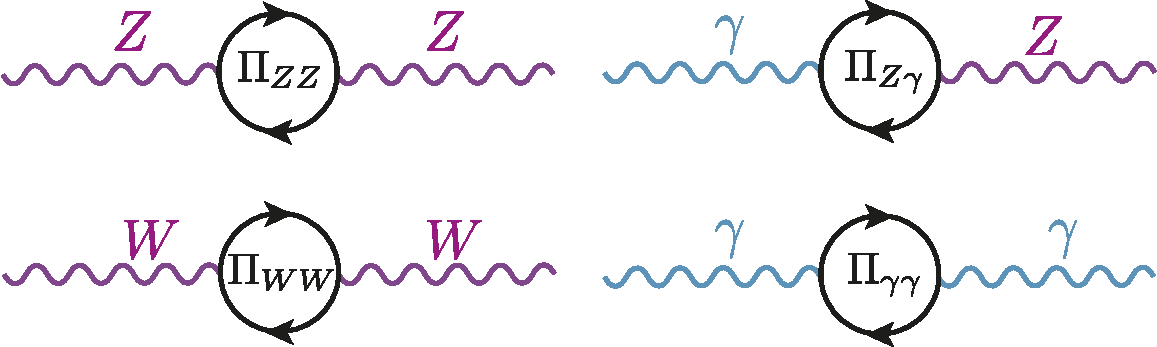
\includegraphics[width=0.75\linewidth]{./figures/oblique_corrections}
	\caption{The oblique corrections, are radiative correction with electroweak gauge bosons propagators. Namely vacuum polarisations of the $Z$, $W^\pm$ and $\gamma$ bosons. }  \label{fig:oblique}
\end{figure}
%%%%
%%%%
The 1-loop correction to the $\rho$ parameter is given in terms of the ~$\Pi_{VV}$  by
\begin{equation}
\Delta \rho = \frac{\Pi_{WW}(0)}{m_W^2}- \frac{\Pi_{ZZ}(0)}{m_Z^2}
\end{equation}
Where the dominant contributions are given by~\cite{EINHORN1981146}
\begin{align}
\Delta \rho & = \frac{3 G_F}{8\sqrt{2}\pi^2}\,\left((m_t^2+m_b^2)-\frac{2m_t^2m_b^2}{m_t^2-m_b^2}\ln \frac{m_t^2}{m_b^2} \right)+\dots.
\label{eq:deltarho}
\end{align}
Since $m_b\ll m_t$, the correction is non-vanishing, and~\eqref{eq:deltarho} shows clearly how the radiative corrections are proportional to the spurions of the custodial symmetry. However, this radiative correction is absorbed into the SM definition of $\rho$, i.e. the $\MSbar$ definition of the $\rho$-parameter~$\rho^{\MSbar}$.
\par One can study  new physics~(NP) effects that violates custodial symmetry, by looking at deviations from $\rho=1$ from it. Given the experimentally measured value of~$\rho$~\eqref{eq:rhoexp} many NP models violating custodial symmetry can already be excluded. Nevertheless, $\rho$ alone does not capture the full story of~EWPO's. For instance, adding a new quark doublet would not necessarily violate the custodial symmetry though it still can be excluded by EWPO. It is hence useful to introduce new parameters known as \textbf{Peskin-Takeuchi parameters}~\cite{PhysRevLett.65.964,Peskin91estimationof,peskin1995introduction}
\begin{align}
	S &:=\frac{4 c_W^2 s_W^2}{\alpha} \left[ \frac{\Pi_{ZZ}^{\NP} (m_Z^2)- \Pi_{ZZ}^{\NP} (0)}{m_Z^2}  - \frac{c_W^2-s_W^2}{c_Ws_W}\,\frac{\Pi_{Z\gamma}^\NP(m_Z^2)}{m_Z^2}-\frac{\Pi_{\gamma\gamma}^\NP(m_Z^2)}{m_Z^2}\right],  \nonumber \\
	T &:=\frac{\rho^{\MSbar}-1}{\alpha}  = \frac{1}{\alpha} \left[ \frac{\Pi^\NP_{WW}(0)}{m_W^2}- \frac{\Pi^\NP_{ZZ}(0)}{m_Z^2} \right] , \\
	U&:= \frac{4 s_W^2}{\alpha} \left[ \frac{\Pi_{WW}^{\NP} (m_W^2)- \Pi_{WW}^{\NP} (0)}{m_W^2}   - \frac{c_W}{s_W}\,\frac{\Pi_{Z\gamma}^\NP(m_Z^2)}{m_Z^2}-\frac{\Pi_{\gamma\gamma}^\NP(m_Z^2)}{m_Z^2}\right] -S .\nonumber 
\end{align}
The NP contributions to the EW vacuum polarisations $\Pi_{VV}^{\NP}(p^2)$) could either come from loop or tree-level effects. Typically both $T$ and $U$ are related to custodial symmetry violation. However, $U$ has an extra suppression factor of $m_\NP^2/m_Z^2$ compared to $T$ and $S$. The most recent fit result for these parameters is~\cite{Zyla:2020zbs}
\begin{align}
	S &=-0.01\pm0.10,  \nonumber \\
	T &= 0.03\pm0.13, \\
	U&:= 0.02\pm0.11.\nonumber 
\end{align}
But since $T$ and $S$ tend to give stronger constraint on NP, due to the suppression factor of $U$. One can preform a two-parameter fit of $S$ and $T$ setting $U=0$, thas shown in~\autoref{fig:stubound}, with the numerical values~\cite{Zyla:2020zbs}, \\
 \begin{align}
 	S &=0.00\pm0.07,  \nonumber \\
 	T &= 0.05\pm0.06.
 \end{align}
%%%%
\begin{figure}[t]
	\centering
	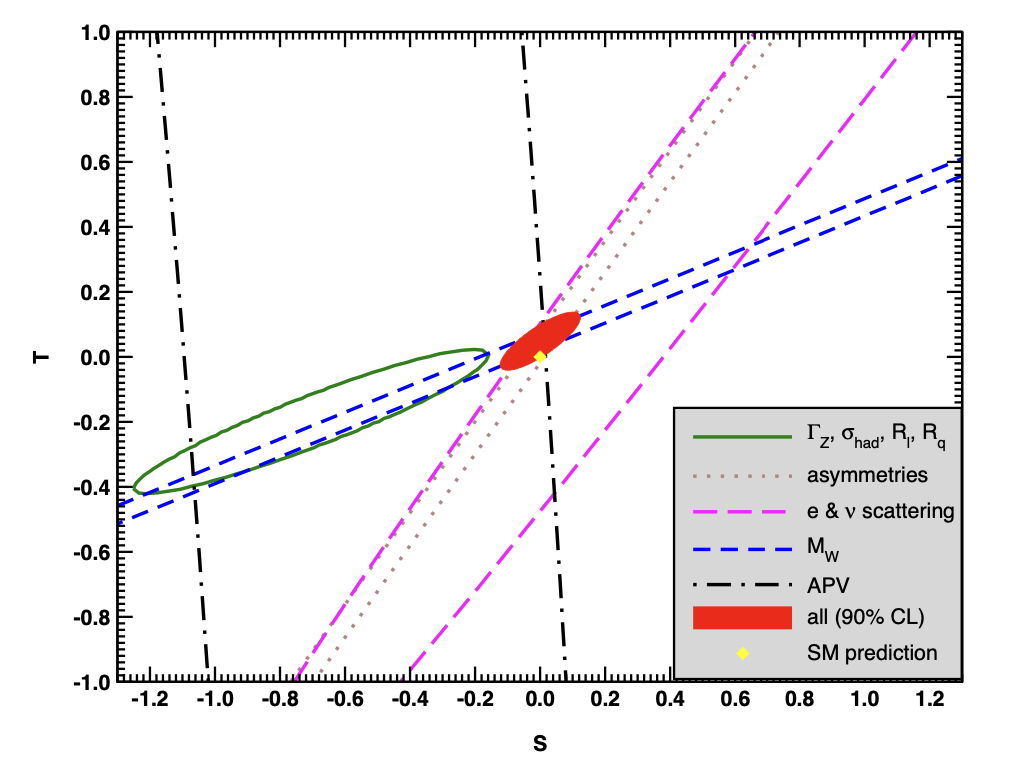
\includegraphics[width=0.65\linewidth]{./figures/stu-pdg}
	\caption{ Fit results from various EWPO's for $T$ and $S$ setting $U=$. The contours show $1\,\sigma$ contours~(39.35\% for closed contours and 68\% for the rest). This plot is obtained from the PDG~\cite{Zyla:2020zbs}  }  \label{fig:stubound}
\end{figure}
%%%%
%%%%
The Peskin-Takeuchi parameters are important in constraining effective operators in the Higgs sector , namely
 \begin{align}
 \hat{O}_S &= \phi^\dagger \sigma_i \phi W^i_{\mu \nu} B^{\mu \nu}, \nonumber \\
\hat{O}_T &= |\phi^\dagger D_\mu \phi|^2.
\end{align}
For example, $\hat{O}_S$ appears in Technicolour models causing large deviations of $S$ compared to its measured value~\cite{GOLDEN19913,HOLDOM199088,ALTARELLI19923,PhysRevLett.65.964}. Moreover, The constraints on $T$ parameter is important for top mass generation ans well as modifications to~$Z  b \bar{b}$ coupling in such models~\cite{PhysRevLett.69.575,Simmons:1995df}. We will revisit the $\hat{O}_T$ when we discuss the Higgs and effective field theories in section \la{update here}.
